
\begin{frame}
    \frametitle{Generator matrix - Steady state probabilities}
    \centering
    
    \begin{tikzpicture}[-, node distance = 0.7cm, auto, every node/.style={scale=0.6}]
        \node[state] (one) {(0,0)};
        \node[state, right=1.5cm of one] (two) {(0,1)};
        \node[state, right=1.5cm of two] (three) {(0,2)};
        \node[state, right=1.5cm of three] (four) {(0,3)};
        \node[state, right=1.5cm of four] (five) {(0,4)};
        \node[state, below=of three] (three_one) {(1,2)};
        \node[state, below=of three_one] (three_two) {(2,2)};
        \node[state, below=of four] (four_one) {(1,3)};
        \node[state, below=of four_one] (four_two) {(2,3)};
        \node[state, below=of five] (five_one) {(1,4)};
        \node[state, below=of five_one] (five_two) {(2,4)};
        \draw[every loop]
            (one) edge[bend left] node {\( \lambda_1 + \lambda_2 \)} (two)
            (two) edge[bend left] node [above] {\( \mu \)} (one)
            (two) edge[bend left] node {\( \lambda_1 + \lambda_2 \)} (three)
            (three) edge[bend left] node [above] {\( 2\mu \)} (two)
            (three) edge[bend left] node {\( \lambda_1 \)} (four)
            (four) edge[bend left] node [above] {\( 3\mu \)} (three)
            (four) edge[bend left] node {\( \lambda_1 \)} (five)
            (five) edge[bend left] node [above] {\( 3\mu \)} (four)
            (three) edge[bend left] node {\( \lambda_2 \)} (three_one)
            (three_one) edge[bend left] node {\( 2\mu \)} (three)
            (three_one) edge[bend left] node {\( \lambda_1 \)} (four_one)
            (four_one) edge[bend left] node [above] {\( 3\mu \)} (three_one)
            (four_one) edge[bend left] node {\( \lambda_1 \)} (five_one)
            (five_one) edge[bend left] node [above] {\( 3\mu \)} (four_one)
            (four) edge node {\( \lambda_2 \)} (four_one)
            (five) edge node {\( \lambda_2 \)} (five_one)
            (three_one) edge[bend left] node {\( \lambda_2 \)} (three_two)
            (three_two) edge[bend left] node {\( 2\mu \)} (three_one)
            (four_one) edge node {\( \lambda_2 \)} (four_two)
            (five_one) edge node {\( \lambda_2 \)} (five_two)
            (three_two) edge[bend left] node {\( \lambda_1 \)} (four_two)
            (four_two) edge[bend left] node [above] {\( 3\mu \)} (three_two)
            (four_two) edge[bend left] node {\( \lambda_1 \)} (five_two)
            (five_two) edge[bend left] node [above]  {\( 3\mu \)} (four_two)
            ;
    \end{tikzpicture}
    \vspace{0.5cm}

    \tiny
    \renewcommand{\arraystretch}{1.5}
    \begin{tabular}{c|c|c|c|c|c|c|}
        \multicolumn{1}{c}{\textbf{From \textbackslash To}}
        & \multicolumn{1}{c}{(0,0)} & 
        \multicolumn{1}{c}{(0,1)} & \multicolumn{1}{c}{(0,2)} & 
        \multicolumn{1}{c}{} & \multicolumn{1}{c}{(2,3)} &
        \multicolumn{1}{c}{(2,4)} \\

        \multicolumn{1}{c}{} & \multicolumn{1}{c}{} & \multicolumn{1}{c}{} &
        \multicolumn{1}{c}{} & \multicolumn{1}{c}{} & \multicolumn{1}{c}{} & 
        \multicolumn{1}{c}{} \\

        \cline{2-7}
        (0,0) & \(-\lambda_1 - \lambda_2\) & \(\lambda_1 + \lambda_2\) & 0 & \(\dots\) & 0 & 0 \\
        \cline{2-7}
        (0,1) & \(\mu\) & \(-\mu - \lambda_1 - \lambda_2\) & \(\lambda_1 + \lambda_2\) & \(\dots\) & 0 & 0 \\
        \cline{2-7}
        (0,2) & 0 & \(2\mu\) & \(-2\mu - \lambda_1 - \lambda_2\) & \(\dots\) & 0 & 0 \\
        \cline{2-7}
        & \(\vdots\) & \(\vdots\) & \(\vdots\) & \(\ddots\) & \(\vdots\) & \(\vdots\) \\
        \cline{2-7}
        (2,3) & 0 & 0 & 0 & \(\dots\) & \(-\lambda_1 - 3\mu\) & \(\lambda_1\) \\
        \cline{2-7}
        (2,4) & 0 & 0 & 0 & \(\dots\) & \(3\mu\) & \(-3\mu\) \\
        \cline{2-7}
    \end{tabular}
\end{frame}


\begin{frame}
    \frametitle{Generator matrix - Steady state probabilities}

    \begin{equation*}
        \pi =
        \begin{bmatrix}
            \pi_{(0,0)} & \pi_{(0,1)} & \pi_{(0,2)} & \dots & \pi_{(2,3)} & 
            \pi_{(2,4)} 
        \end{bmatrix},
        \qquad \sum \pi_{(u,v)} = 1
    \end{equation*}

    \begin{tikzpicture}[-, node distance = 0.7cm, auto, every node/.style={scale=0.6}]
        \node[state] (one) {\(\pi_{(0,0)}\)};
        \node[state, right=1.5cm of one] (two) {\(\pi_{(0,1)}\)};
        \node[state, right=1.5cm of two] (three) {\(\pi_{(0,2)}\)};
        \node[state, right=1.5cm of three] (four) {\(\pi_{(0,3)}\)};
        \node[state, right=1.5cm of four] (five) {\(\pi_{(0,4)}\)};
        \node[state, below=of three] (three_one) {\(\pi_{(1,2)}\)};
        \node[state, below=of three_one] (three_two) {\(\pi_{(2,2)}\)};
        \node[state, below=of four] (four_one) {\(\pi_{(1,3)}\)};
        \node[state, below=of four_one] (four_two) {\(\pi_{(2,3)}\)};
        \node[state, below=of five] (five_one) {\(\pi_{(1,4)}\)};
        \node[state, below=of five_one] (five_two) {\(\pi_{(2,4)}\)};
        \draw[every loop]
            (one) edge[bend left] node {} (two)
            (two) edge[bend left] node {} (one)
            (two) edge[bend left] node {} (three)
            (three) edge[bend left] node {} (two)
            (three) edge[bend left] node {} (four)
            (four) edge[bend left] node {} (three)
            (four) edge[bend left] node {} (five)
            (five) edge[bend left] node {} (four)
            (three) edge[bend left] node {} (three_one)
            (three_one) edge[bend left] node {} (three)
            (three_one) edge[bend left] node {} (four_one)
            (four_one) edge[bend left] node {} (three_one)
            (four_one) edge[bend left] node {} (five_one)
            (five_one) edge[bend left] node {} (four_one)
            (four) edge node {} (four_one)
            (five) edge node {} (five_one)
            (three_one) edge[bend left] node {} (three_two)
            (three_two) edge[bend left] node {} (three_one)
            (four_one) edge node {} (four_two)
            (five_one) edge node {} (five_two)
            (three_two) edge[bend left] node {} (four_two)
            (four_two) edge[bend left] node {} (three_two)
            (four_two) edge[bend left] node {} (five_two)
            (five_two) edge[bend left] node {} (four_two)
            ;
    \end{tikzpicture}

    \Large
    \begin{equation*}
        \frac{d \pi}{dt} = \pi Q = 0
    \end{equation*}

\end{frame}



\begin{frame}
    \frametitle{Generator matrix - Steady state probabilities}

    \centering
    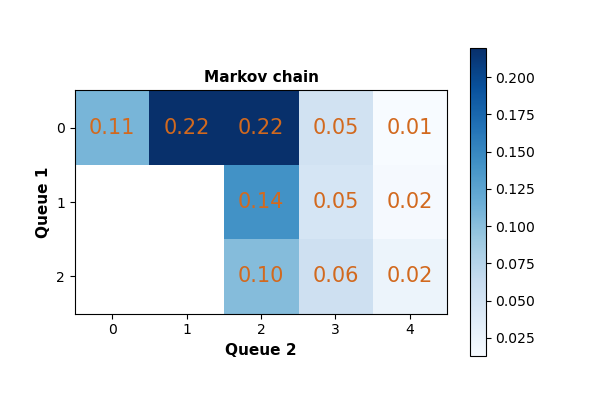
\includegraphics[scale=0.39, trim= 0 0 100 0, clip]{Bin/state_probs_comparison/markov.png}
    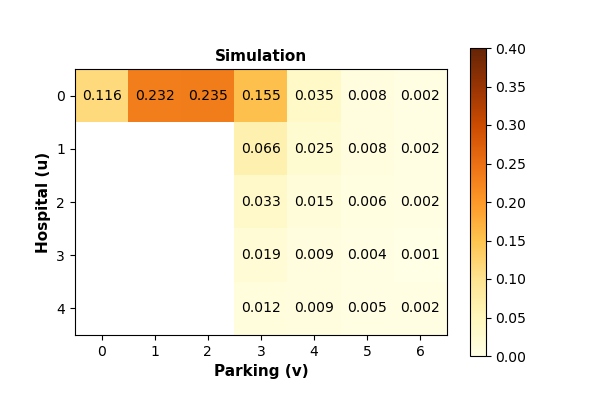
\includegraphics[scale=0.39]{Bin/state_probs_comparison/simulation.png}

\end{frame}